% Pré-requis : afin de tirer bénéfice de ces séances de C/TD/TP, vous devez au préalable maîtriser les savoirs et savoir-faire suivant :
% - connaître les notions de : variable propositionnelle, valuation, modèle, conséquence logique, (in)satisfiabilité
% - utiliser correctement les connecteurs logiques pour la modélisation de problèmes
% - évaluer une conséquence logique, rechercher d'un modèle, tirer les bonnes conclusions quant à  leur (in)existence

% Objectifs : 
% À l'issue de ces séances, vous devrez être capable de transformer un problème de type combinatoire (dont le sudoku est un exemple typique) en un problème de satisfiabilité d'un ensemble de formules logiques. Pour cela , vous devrez tirer parti des facilités expressives offertes par les connecteurs généralisés dans \touist. Puis, vous devez pouvoir, à partir des modèles obtenus (ou de leur absence) conclure quant aux solutions du problème concret dont vous serez partis.

\subsection{Utilisation du prouveur}
\subsubsection{Vérifier si une formule admet un modèle (= est satisfiable)}
\begin{enumerate}
\item Saisissez la formule $p\vee q\rightarrow p$
\item Vérifiez, en bas à droite, que le sélecteur est sur "SAT" puis cliquez sur Solve.
\item Le solveur vous indique un modèle de la formule : la valuation $v(p)=0$ et $v(q)=0$. En cliquant sur "Next" vous accédez aux autres modèles (s'il y en a). Les coches "True" et "False" permettent de n'afficher que les propositions à True ou à False. 
\item Retour à l'édition.
\item Saisissez la formule $p\wedge\neg p$. Solve. Vous avez une pop-up qui vous informe qu'il n'y a pas de modèle : la formule est insatisfiable. 
\item Saisissez "p$\vee \neg$ p". Solve : il y a deux modèles sur deux possibles, normal la formule est valide !
\end{enumerate}
Exercice : trouvez les modèles de $(p \vee q \vee r) \wedge (p \rightarrow \neg q) \wedge (q \rightarrow \neg r) \wedge (r\rightarrow \neg p)$. Vérifiez que dans chacun une seule proposition est vraie. 

\subsection{Vérifier si une formule est valide}
Rappel : une formule valide est vraie dans tous les modèles. 

Si l'on saisit une formule et qu'on veut savoir si elle est valide, on doit vérifier qu'elle a autant de modèle qu'il y en a de possibles ! (pas pratique).

On procède indirectement, par réfutation. Si elle est valide, sa négation sera insatisfiable. On teste donc sa négation, ici $\neg(p\vee \neg p)$. Faites-le. Vous constatez qu'il n'y a pas de solution, donc la formule $p\vee \neg p$ est valide ! \\

Exercice : Vérifiez que $pluie \wedge (pluie \rightarrow routeMouillee) \wedge (routeMouillee\rightarrow danger) \rightarrow danger$ est valide. 
\subsection{Vérifier si un ensemble de formules admet un modèle (= est satisfiable)}
On saisit simplement les formules de l'ensemble, les unes au-dessus des autres, puis Solve. \\
Exercice : Vérifiez que l'ensemble $\mathit{cafe\vee the, \neg the}$ est satisfiable. Quel unique modèle admet-il ? 
\subsection{Vérifier si une formule $C$ est conséquence logique d'un ensemble $H$ de formules}
Supposons que $H=\{H1,\cdots,Hn\}$ est un ensemble de $n$ hypothèses.\\
Là encore, il serait fastidieux de vérifier que $C$ est vraie dans tous les modèles de $H$. Là encore on procède indirectement en utilisant le théorème : 
\[H\models C \mbox{ si et seulement si } H\cup\{\neg C\}\mbox{ est insatisfiable}\]
autrement dit, pour vérifier si $H\models C$, on va tester si les formules $H1$, $H2$,\ldots, $Hn$, $\neg C$ prises \emph{toutes ensemble} sont satisfiables. Si ça n'est pas le cas on pourra conclure que $H\models C$. Si c'est pas le cas, on aura au moins un contre-modèle ($\sim$ un contre-exemple) qui nous dira dans quelle situation on a les hypothèses vraies et la conclusion fausse.

Exercice : Testez les conséquences suivantes et donnez un contre-modèle quand elle ne sont pas correctes : 
\begin{itemize}
\item $f\rightarrow m, f \models m$
\item $f\rightarrow m, r\rightarrow m, \neg f\wedge \neg r \models \neg m$\\
(f=j'ai de la fièvre, r=j'ai des rougeurs, m=je suis malade)
\item $f\rightarrow m, r\rightarrow m, \neg m\models \neg f\wedge \neg r $


\item On suppose que l’on a l'ensemble $H$ de règles et faits suivants :

\begin{enumerate}
\item Si le patient a la rougeole, il a de la fièvre.
\item Si le patient a une hépatite, mais pas la rougeole, il a le teint jaune.
\item Si le patient a de la fièvre ou le teint jaune, il a une hépatite ou la rougeole.
\item Le patient n’a pas le teint jaune.
\item Le patient a de la fièvre.
\end{enumerate}

Vérifiez que dans tous les modèles de $H$, la variables $r$ (correspondant à "le patient a la rougeole") est à "vrai". Vérifiez que $H \models r$.
\end{itemize}
\newpage
\section{Les connecteurs généralisés : $\bigwedge_{i \in A}$ et $\bigvee_{i \in A}$}

Pour simplifier l'écriture de certaines formules, il est possible d'utiliser des connecteur logiques généralisés.
Par exemple, considérons une grille de \emph{carré latin}\footnote{comme un sudoku sans la contrainte sur les régions : 1 chiffre par case qui apparaît une seule fois par ligne et par colonne.} $4\times 4$ à résoudre :
\begin{center}
\texttt{
\begin{tabular}{|c|c|c|c|}
	\hline
	~ & ~ & 1 & ~ \\ \hline
	~ &~ & ~ & 2 \\ \hline
	4 & ~ & ~ & ~ \\ \hline
	~ & ~ & 3 &  \\ \hline
\end{tabular}
}\\
\end{center}

Pour chacune des cases, nous définissons quatre variables propositionnelles correspondant aux quatre valeurs possibles $\{1,2,3,4\}$ qu'on écrit aussi $[1..4]$. Ainsi, $p(i,j,k)$ représentera la proposition "La case de coordonnées $(i,j)$ contient la valeur $k$".\\

Pour imposer que la case de coordonnées (2,1) contient l'une des quatre valeurs possibles, nous pouvons utiliser la formule : \\
\[\texttt{p(2,1,\hl{1}) or p(2,1,\hl{2}) or p(2,1,\hl{3}) or p(2,1,\hl{4})}\]

Cette succession de $\vee$ ou seul l'un des indices (surligné) varie peut être condensée en utilisant le $\bigvee$ : 
\[\bigvee_{k\in [1..4]} \texttt{p(2,1,\hl{k})} \]
qui signifie donc "la case (2,1) contient l'une des quatre valeurs possibles", ou "pour l'une au moins des quatre valeurs possibles, cette valeur est dans la case (1,2)". \\

\noindent Remarquez l'analogie avec le $\Sigma$ mathématique avec lequel une expression telle que : 
\[f(x,1)+f(x,2)+\cdots+f(x,10)\]
serait condensée en :
\[\sum_{k\in[1..10]} f(x,k)\]


Nous voulons maintenant exprimer que \emph{toutes} les cases de la ligne 2 (cases de coordonnées (2,x)) contiennent l'une des quatre valeurs possibles : 

\[\bigvee_{k\in [1..4]} \texttt{p(2,\hl{1},k)} \wedge \bigvee_{k\in [1..4]} \texttt{p(2,\hl{2},k)}\wedge
\bigvee_{k\in [1..4]} \texttt{p(2,\hl{3},k)} \wedge
\bigvee_{k\in [1..4]} \texttt{p(2,\hl{4},k)}\] 

Pour cela, nous utilisons le $\bigwedge$ en faisant varier l'indice surligné et obtenons : 
\[\bigwedge_{j\in [1..4]}\bigvee_{k\in [1..4]} \texttt{p(2,\hl{j},k)}\]

Ce qui peut se lire "pour chaque case de la ligne 2, pour au moins une valeur de [1..4], cette valeur est dans la case". \\

Afin maintenant d'exprimer la même chose pour chaque ligne, nous généralisons en faisant varier le numéro de ligne : 

\[\bigwedge_{j\in [1..4]}\bigvee_{k\in [1..4]} \texttt{p(\hl{1},j,k)}\wedge \bigwedge_{j\in [1..4]}\bigvee_{k\in [1..4]} \texttt{p(\hl{2},j,k)}\wedge \bigwedge_{j\in [1..4]}\bigvee_{k\in [1..4]} \texttt{p(\hl{3},j,k)}\wedge \bigwedge_{j\in [1..4]}\bigvee_{k\in [1..4]} \texttt{p(\hl{4},j,k)}\]

soit, en utilisant à nouveau le $\bigwedge$ :

\[\bigwedge_{i\in [1..4]}\bigwedge_{j\in [1..4]}\bigvee_{k\in [1..4]} \texttt{p(\hl{i},j,k)}\]
Qui peut se lire "Pour chaque case (i,j) de la grille, il y a au moins une valeur parmi les quatre possibles qui y figure". \\

\noindent NB : sans ces facilités d'écriture, il aurait fallu 64 propositions et 63 connecteurs pour écrire la même chose. \\

Cette écriture est possible dans \touist en utilisant des variables \texttt{\$i}, \texttt{\$j} et \texttt{\$k}.

Ce qui donne : 
\begin{verbatim}
1 |  bigand $i in [1..4]:
2 |    bigand $j in [1..4]:
3 |      bigor $k in [1..4]:
4 |        p($i,$j,$k)
5 |      end
6 |    end
7 |  end
\end{verbatim}

% \begin{center}
% 	\begin{tabular}{cV{4cm}} \toprule
% 		Logique propositionnelle & Langage \touist \\ \midrule
% 		Pour $n\in \mathbb{N}^{*}$, $\underset{i\in [1..n]}{\bigwedge}p_{i}$ & 
% 		\begin{verbatim}
% 		bigand $i in [1..n]:
% 		    p($i)
% 		end
% 		\end{verbatim}
% 		\\ \hline
% 		Pour $n\in \mathbb{N}^{*}$, $\underset{i\in [1..n]}{\bigvee}p_{i}$ & 
% 		\begin{verbatim}
% 		bigor $i in [1..n]:
% 		    p($i)
% 		end
% 		\end{verbatim}
%          \\ \hline
% 	\end{tabular}
% \end{center}

Exercice : Résoudre le Sudoku $4\times 4$ donné en exemple en utilisant les connecteurs généralisés :
\begin{itemize}
	\item Écrire une formule qui décrit l'état initial de la grille ci-dessus ;
    \item Recopier la formule qui impose que chaque cellule contienne \textbf{au moins} une valeur de $[1..4]$ ;
	\item Écrire une formule qui impose que chaque cellule contienne \textbf{au plus} une valeur parmi $[1..4]$ 
Indice : si une cellule contient une valeur alors elle n'en contient pas d'autre. Par exemple, pour exprimer que la case $(1,4)$ contient seulement un 3, il faut parvenir à écrire une formule disant que toute autre valeur que 3 est absente de la case $(2,3)$, en formule : 
\[\texttt{p(1,4,\hl{3}) => (not p(1,4,\hl{1}) and not p(1,4,\hl{2}) and not p(1,4,\hl{4})})\]
\end{itemize}
On remarque qu'en partie droite de cette implication, on retrouve toutes les valeurs possibles \emph{sauf} 3. Le langage de \touist permet d'exprimer cela de manière compacte grâce à la clause \texttt{when}: 

\[\texttt{p(1,4,3) => bigand \$k in [1..4] \hl{when \$k!= 3}: not p(1,4,\$k)}\]

De manière générale dans : 
\begin{verbatim}
   ....
   bigand $i in [1..4] when $i != $j : ....
\end{verbatim}
(\$i ne prendra pas la valeur qu'a \$j)

Il ne reste plus qu'à appliquer ce principe à toutes les cases\ldots

\begin{itemize}
    \item Dans la même veine, écrire une formule qui interdit deux valeurs identiques dans les cellules d'une même ligne ;
    \item Faire de même pour les colonnes ;\\
    Muni(e) de ces formules résolvez le carré latin du dessus, et vérifiez qu'il admet plusieurs solutions. 
    \item (Difficile) Passons au sudoku $4\times 4$ : sachant que, dans \touist, il est possible d'effectuer des opérations arithmétiques sur des variables entières (par exemple \texttt{p(\$u+\$i,\$v+\$j,\$k)}), écrire une formule qui interdit deux valeurs identiques dans les cellules d'une même région.\\
    Vérifiez que le carré latin peut être résolu avec les règles du sudoku et n'admet alors plus qu'une solution. 
    
\item Modifiez vos formules pour traiter un sudoku classique ($9\times 9$), et résolvez \href{http://puzzling.stackexchange.com/questions/252/how-do-i-solve-the-worlds-hardest-sudoku}{celui-ci par exemple} (l'un des plus difficiles au monde). 
\end{itemize}

\section{Les ensembles}

Nous avons vu comment définir des variables entières utilisées comme indices.
Nous allons maintenant voir comment utiliser des ensembles génériques pour construire des formules avec les connecteurs généralisés. L'intérêt sera notamment de séparer les règles de résolution d'un problème qui seront définies par des formules permettant de résoudre tout problème de même nature, et des ensembles définissant un problème particulier. Par exemple, dans le cas du Sudoku, les formules permettront de résoudre n'importe quel Sudoku, et les ensembles définiront la grille de Sudoku que nous souhaitons résoudre en particulier.\\

L'onglet "Sets" nous permet de définir de tels ensembles. Par exemple, nous souhaitons remplacer les chiffres contenus dans les cases du Sudoku par des lettres. Nous pouvons alors définir l'ensemble $L=\{A,B,C,D\}$ par \texttt{\$L=[A,B,C,D]} dans l'onglet "Sets" et remplacer \texttt{\$k in [1..4]} par \texttt{\$k in \$L} dans les formules.\\

Exercice : résoudre le sudoku $4\times 4$ : 

\begin{center}
\texttt{
\begin{tabular}{|c|c|c|c|}
	\hline
	A & B & ~ & ~ \\ \hline
	~ & D & ~ & ~ \\ \hline
	~ & ~ & A & ~ \\ \hline
	~ & ~ & C & B \\ \hline
\end{tabular}
}\\
\end{center}

Exercice : Coloration de cartes.\\

Le théorème des 4 couleurs, qui fut conjecturé en 1852 par Francis Guthrie, affirme qu'on peut colorer toute carte géographique en utilisant seulement 4 couleurs tout en veillant à ce que deux pays limitrophes reçoivent des couleurs différentes. Il a été (enfin) démontré en 1976 par Appel et Haken. La démonstration a exigé l'usage de l'ordinateur pour étudier les 1478 cas critiques (plus de 1200 heures de calcul à l'époque). \\

Soit l'ensemble de pays européens (on ne les considère pas tous, mais vous pouvez) : \\
\begin{multline}
P = \{Portugal, Espagne, France, Italie, Suisse, Belgique, PaysBas, Pologne, Autriche,\\ RepTcheque, Slovenie, Croatie, Luxembourg, Allemagne\}
\end{multline}
Formalisez le problème de la coloration de pays : 
\begin{itemize}
\item Chaque pays reçoit une et une seule couleur
\item Deux pays limitrophes reçoivent des couleurs différentes
\item Si A est limitrophe avec B, alors B l'est avec A. 
\end{itemize}
Vous définirez l'ensemble $P$ des pays et l'ensemble $C$ des couleurs (disons $\{Jaune, Rouge, Vert, Bleu\})$. \\

\noindent Vous utiliserez les propositions : 
\begin{itemize}
\item \texttt{r(p,c)} : "le pays p reçoit la couleur c"
\item \texttt{l(p1,p2)} : "le pays p1 est limitrophe avec le pays p2"
\end{itemize}

NB : en cas de doute, pour savoir lesquels de ces pays sont limitrophes, consultez \href{https://upload.wikimedia.org/wikipedia/commons/6/6a/Europe_countries_map_fr.png}{cette carte}. \\

Utilisez \touist pour découvrir une solution à quatre couleurs. Puis testez s'il existe une solution à trois couleurs. 
\newpage
\section{Traitement des aspects dynamiques}\label{sec:prob}
Jusqu'ici, nous avons traité de problèmes combinatoires statiques : la solution ne nécessite pas d'ordonner une série d'éléments contrairement à ce qui se passe par exemple dans un jeu où il ne suffit pas de savoir quels coups seront joués mais aussi dans quel ordre. 

Un système qui nécessite la prise en compte de quelque chose (à définir) qui évolue est appelé \emph{système dynamique}. Le système évolue donc en passant d'un \emph{état} à un autre, chaque état pouvant être décrit à l'aide d'une formule logique\footnote{On parle aussi de système de transition ou de système à état discret.}. Une des façons d'en rendre compte est de rendre explicite le déroulement du temps, en général un temps discret qui s'incrémente de 1 entre deux états. Mais on peut aussi en rendre compte tout simplement en nommant les états successifs, le passage du temps étant marqué par le nom des actions effectuées. 

\textsc{BlocksWorld} est un monde simplifié pour étudier des problèmes de
planification qu'un robot doit résoudre dans le monde réel. La simplification
concerne les objets à manipuler (des blocs empilés, d'où le nom) et les
opérations que le robot peut effectuer (dans notre cas, déplacer un bloc d'une
pile sur une autre). 
%-------------------------------------------
\subsection{Modélisation du domaine}\label{sec:form_dom}

\textsc{BlocksWorld} est un monde très carré: un ensemble de \emph{blocs} empilés, ce
qui donne un ensemble de tours plus ou moins élevées de blocs. En plus, ces
tours ne peuvent pas se trouver n'importe où, mais uniquement sur des
\emph{tables}. Nous parlons d'\emph{emplacement} pour désigner aussi bien un bloc qu'une table.

Il y a des actions qui modifient le \textsc{BlocksWorld} et donc l'état du monde 
dépend du temps. Par contre, il y a aussi des propriétés immuables, par exemple, être un bloc ou une table.

Dans un premier temps, nous supposons que notre monde est composé de quatre
blocs \texttt{B1,...,B4} et deux tables \texttt{T1,T2}. Si nécessaire, nous apporterons
des modifications. 

Pour modéliser le fait qu'un bloc \texttt{b} se trouve sur un emplacement \texttt{p} (c'est à
dire, une table ou un autre bloc), nous utilisons la famille de variables indexées
\texttt{Sur}. Puisque la position dépend aussi du temps \texttt{s}, on obtient donc
des propositions de la forme \texttt{Sur(b,p,s)}. Le temps est discret; pour cela,
nous parlons aussi d'\emph{état} ou de \emph{situation}. Nous le modélisons par un nombre
naturel. Nous considérons d'abord un intervalle \texttt{[0..9]}.

Pour commencer, nous formalisons quelques exigences concernant \texttt{Sur}. Vous utiliserez des ensembles (Sets) pour spécifier les différentes valeurs (intervalle temporel, nom des blocs et autres). 

\begin{exo}\label{ex:unique_sous}
Donnez une formule qui exprime qu'à tout moment, au plus un emplacement peut se
  trouver \emph{sous} un bloc. Autrement dit, un bloc ne peut pas reposer sur
  plusieurs supports.
\end{exo}
%......................................................................
\begin{figure}[h]
\begin{subfigure}[b]{0.5\textwidth}
\centering
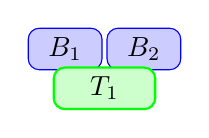
\begin{tikzpicture}[scale=0.5,auto,
block/.style ={rectangle, draw=blue, fill=blue!20,
  text width=2em, text centered, rounded corners,
  minimum height=1em
},
place/.style ={rectangle, draw=green, thick, fill=green!20,
  text width=3em, text centered, rounded corners,
  minimum height=1em
}]
\node (b1) at (-1,1) [block] {$B_1$};
\node (b2) at (1,1) [block] {$B_2$};
\node (p1) at (0,0) [place] {$T_1$};
\end{tikzpicture}
\caption{}\label{fig:unique_sur}
\end{subfigure}%
%
\begin{subfigure}[b]{0.5\textwidth}
\centering
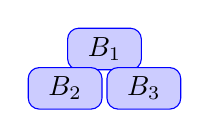
\begin{tikzpicture}[scale=0.5,auto,
block/.style ={rectangle, draw=blue, fill=blue!20,
  text width=2em, text centered, rounded corners,
  minimum height=1em
},
place/.style ={rectangle, draw=green, thick, fill=green!20,
  text width=3em, text centered, rounded corners,
  minimum height=1em
}]
\node (b1) at (0,1) [block] {$B_1$};
\node (b2) at (-1,0) [block] {$B_2$};
\node (b3) at (1,0) [block] {$B_3$};
\end{tikzpicture}
\caption{}\label{fig:unique_sous}
\end{subfigure}%
%
\caption{Configurations illégales}\label{fig:config_illeg}
\end{figure}

\begin{exo}\label{ex:unique_sur_sous_ex} 
Définissez les formules qui décrivent la situation de la
  figure~\ref{fig:unique_sur}. Montrez que cette situation n'est pas
  compatible avec l'exigence de l'exercice~\ref{ex:unique_sur}. Pareil,
  montrez que la figure~\ref{fig:unique_sous} n'est pas compatible avec la
  formule de l'exercice~\ref{ex:unique_sous}.
\end{exo}

\begin{exo}\label{ex:tables}En utilisant un ensemble pour les \emph{tables}, donnez une formule qui exprime qu'une table ne peut pas se trouver sur un  emplacement. Dans un premier temps, les tables sont \texttt{T1} et \texttt{T2}.
\end{exo}


Nous nous limitons donc à des situations où il y a, en bas, un nombre de
tables sur lesquelles on peut empiler des blocs, de manière linéaire, comme
dans la figure~\ref{fig:ex3}.
Pourtant, les exigences imposées jusqu'à maintenant (donc l'ensemble des
formules à l'exception des formules pour
l'exercice~\ref{ex:unique_sur_sous_ex}) n'excluent pas des situations
apparemment ``absurdes'' qui ne correspondent pas à une réalité physique.


\begin{exo}\label{ex:sur_asym_satisfiable}
Montrez que, sous les hypothèses formalisées jusqu'à maintenant, il n'est
  pas incohérent que le bloc \texttt{B1} est sur le bloc \texttt{B2} et en même temps
  \texttt{B2} sur \texttt{B1}.
  \end{exo}

  \begin{exo}\label{ex:sur_asym}
  Pour éviter cette situation, donnez une formule qui exprime que \texttt{Sur}
  est asymétrique dans toute situation \texttt{s}. \emph{Rappel:} une relation $R$ est dite
  asymétrique si $\forall x. \forall y. (R(x,y) \to  \lnot R(y,x))$.
\end{exo}

\begin{exo}\label{ex:sur_irrefl}
  Démontrez avec \textsc{\touist} que, pour tout instant \texttt{s}, l'asymétrie
  de \texttt{Sur} implique l'irréflexivité de \texttt{Sur}. \emph{Rappel:} une
  relation $R$ est dite irréflexive si $\forall x. \lnot R(x,x)$.

  \emph{Aide:} vous devez montrer que $A \models I$, où la formule $A$ exprime
  l'asymétrie et la formule $I$ l'irréflexivité de \texttt{Sur}. Trouvez une
  formule contenant $A$ et $I$ qui est insatisfiable si et seulement si $A
  \models I$, et montrez avec \textsc{\touist} que cette formule est
  effectivement insatisfiable.
\end{exo}



\begin{exo}\label{ex:sur_cycl}
Supposons désormais que \texttt{Sur} est asymétrique. Montrez que, même sous
  cette hypothèse, on ne peut pas exclure la situation suivante: \texttt{B1} est sur
  le bloc \texttt{B2}, \texttt{B2} sur \texttt{B3} et \texttt{B3} sur \texttt{B1}.
  \end{exo}
\begin{exo}\label{ex:unique_sur}
Donnez une formule qui exprime qu'à tout moment  \texttt{s} de notre intervalle
  temporel de référence modélisé par la variable \texttt{\$Time}, au plus un bloc peut se
  trouver \emph{sur} un emplacement. Autrement dit, un emplacement ne peut pas porter
  plusieurs blocs.
\end{exo}


\section{Formalisation des actions}\label{sec:form_act}

%......................................................................
\begin{figure}[h]
\begin{subfigure}[b]{0.5\textwidth}
\centering
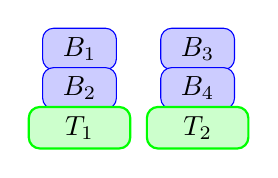
\begin{tikzpicture}[scale=0.5,auto,
block/.style ={rectangle, draw=blue, fill=blue!20,
  text width=2em, text centered, rounded corners,
  minimum height=1em
},
place/.style ={rectangle, draw=green, thick, fill=green!20,
  text width=3em, text centered, rounded corners,
  minimum height=1em
}]
\node (b1) at (0,2) [block] {$B_1$};
\node (b2) at (0,1) [block] {$B_2$};
\node (p1) at (0,0) [place] {$T_1$};
\node (b3) at (3,2) [block] {$B_3$};
\node (b4) at (3,1) [block] {$B_4$};
\node (p2) at (3,0) [place] {$T_2$};
\end{tikzpicture}
\caption{}\label{fig:ex3}
\end{subfigure}%
%
\begin{subfigure}[b]{0.5\textwidth}
\centering
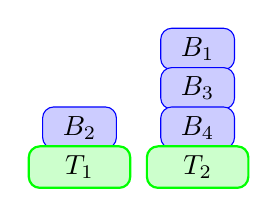
\begin{tikzpicture}[scale=0.5,auto,
block/.style ={rectangle, draw=blue, fill=blue!20,
  text width=2em, text centered, rounded corners,
  minimum height=1em
},
place/.style ={rectangle, draw=green, thick, fill=green!20,
  text width=3em, text centered, rounded corners,
  minimum height=1em
}]
\node (b2) at (0,1) [block] {$B_2$};
\node (p1) at (0,0) [place] {$T_1$};
\node (b1) at (3,3) [block] {$B_1$};
\node (b3) at (3,2) [block] {$B_3$};
\node (b4) at (3,1) [block] {$B_4$};
\node (p2) at (3,0) [place] {$T_2$};
\end{tikzpicture}
\caption{}\label{fig:ex4}
\end{subfigure}%
%
\caption{Dispositions des blocs sur des tables}\label{fig:blocs_tables1}
\end{figure}

%......................................................................

\begin{exo}\label{ex:libre}
Pour faciliter la formalisation des actions, définissez 
  \texttt{Libre($p$,$s$)}, où $p$ est un emplacement et $s$ un état, qui dit que
  dans l'état $s$, il n'y a pas de bloc sur $p$. 
\end{exo}

L'action de notre robot consiste à déplacer un bloc d'un emplacement à un
autre. Pour le décrire, nous introduisons \texttt{Depl(b,p,s)} avec la signification d'un déplacement de $b$ vers l'emplacement $p$, au
moment $s$. Ainsi, le passage de la situation \ref{fig:ex3} à la situation
\ref{fig:ex4} est décrit par \texttt{Depl(B1,B3,0)}, si \ref{fig:ex3} est
la situation initiale, donc au moment $s = 0$.
L'emplacement du bloc $b$ dans l'état $s$ devrait être connu; pour
cela, il serait redondant de rajouter le point de départ de $b$ au prédicat
\texttt{Depl}.

Pour qu'un tel déplacement d'un bloc puisse avoir lieu, quelques conditions
doivent être satisfaites:

\begin{itemize}
\item le bloc $b$ doit être libre (il n'est pas possible de retirer $b$ du
  milieu d'une pile)
\item de même pour l'emplacement $p$;
\item comme mentionné avant, on ne peut pas transporter des tables, mais
  uniquement des blocs.
\end{itemize}

Le déplacement entraîne quelques changements entre l'état actuel (disons $s$)
et l'état suivant ($s + 1$):
\begin{itemize}
\item $b$ est maintenant sur $p$,
\item tandis que $b$ reste libre;
\item et son emplacement précédent est maintenant libre.
\end{itemize}

Il faudra aussi préciser que les blocs qui n'ont pas bougé restent sur leurs
emplacements précédents.

\begin{exo}\label{ex:depl}
Formalisez ces conditions. Vous obtenez une implication de la forme
  \texttt{Depl(b,p,s) $\to \; F_1 \land F_2 \land \dots$}, où les $F_i$
  sont les faits évoqués en haut.  N'oubliez pas les quantifications
  $\bigwedge$ et $\bigvee$ nécessaires.
\end{exo}

\begin{exo}\label{ex:progr}
Nous avons encore besoin d'une propriété de ``progrès'': Le passage d'un
  instant à l'instant suivant est toujours accompagné de l'exécution d'une
  action. Donc, à chaque instant, un bloc est déplacé.
  (Quels résultats obtenez vous sans cette clause?)
\end{exo}

  Pourvu que l'état d'arrivée est satisfiable, sans cette clause, on obtient
  toujours une solution où \texttt{Depl} est faux et on atteint l'état
  d'arrivée ``par magie''.

\section{Expérimentation}\label{sec:exper}

Nous allons maintenant utiliser \textsc{\touist} pour synthétiser un plan
pour atteindre un état, à partir d'un état de départ. L'état de départ est
caractérisé par un nombre de conditions au temps $s = 0$. Pour savoir si un
état est atteignable en $n$ pas (ou moins), vous posez le problème s'il existe
un $s$ dans l'intervalle $0 \dots n$ qui satisfait la condition d'arrivée. 

\begin{exo}\label{ex:exp1}
En partant de la situation initiale de la figure~\ref{fig:ex3}, montrez qu'il existe une
  situation où $B_4$ est sur $B_3$.
  \end{exo}

\begin{exo}\label{ex:exp1_neg}
Étant donnée la situation de la figure~\ref{fig:ex3}, montrez qu'on ne peut pas
  atteindre en 5 pas une situation où $B_2$ est sur $B_4$. 
  \end{exo}

  \emph{Question de réflexion:} Ce résultat n'est pas une preuve
  d'inatteignabilité de l'état pour un nombre arbitraire de pas. Combien de
  configurations a le \textsc{BlocksWorld} avec 2 tables et 4 blocs? Quel est
  le nombre maximal de pas à prendre en compte pour prouver l'inatteignabilité
  d'un état? (N'essayez pas de le faire).

\begin{exo}\label{ex:exp2}
Par contre, si vous rajoutez une troisième table $T_3$, il est bien possible
  d'atteindre la situation où $B_2$ est sur $B_4$.
    \end{exo}


\begin{exo}\label{ex:exp3}
Vérifiez qu'on ne peut, en $x$ étapes passer de la situation de la figure \ref{fig:ex5a} à la situation \ref{fig:ex5b} pour $x$  valant 3,4,5 ou plus. Ajoutez une table et vérifiez qu'il existe une solution en 5 étapes. 
%......................................................................
\begin{figure}[h]
\begin{subfigure}[b]{0.5\textwidth}
\centering
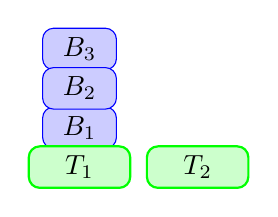
\begin{tikzpicture}[scale=0.5,auto,
block/.style ={rectangle, draw=blue, fill=blue!20,
  text width=2em, text centered, rounded corners,
  minimum height=1em
},
place/.style ={rectangle, draw=green, thick, fill=green!20,
  text width=3em, text centered, rounded corners,
  minimum height=1em
}]
\node (b2) at (0,1) [block] {$B_1$};
\node (p1) at (0,0) [place] {$T_1$};
\node (b1) at (0,3) [block] {$B_3$};
\node (b3) at (0,2) [block] {$B_2$};
\node (p2) at (3,0) [place] {$T_2$};
\end{tikzpicture}
\caption{}\label{fig:ex5a}
\end{subfigure}%
%
\begin{subfigure}[b]{0.5\textwidth}
\centering
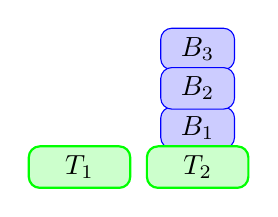
\begin{tikzpicture}[scale=0.5,auto,
block/.style ={rectangle, draw=blue, fill=blue!20,
  text width=2em, text centered, rounded corners,
  minimum height=1em
},
place/.style ={rectangle, draw=green, thick, fill=green!20,
  text width=3em, text centered, rounded corners,
  minimum height=1em
}]
\node (b2) at (3,1) [block] {$B_1$};
\node (p1) at (0,0) [place] {$T_1$};
\node (b1) at (3,3) [block] {$B_3$};
\node (b3) at (3,2) [block] {$B_2$};
\node (p2) at (3,0) [place] {$T_2$};
\end{tikzpicture}
\caption{}\label{fig:ex5b}
\end{subfigure}%
%
\caption{Problème à 3 blocs}\label{fig:blocs_tables2}
\end{figure}

%......................................................................
  \end{exo}

\begin{exo}\label{ex:exp4}
Quelle est la longueur du plan optimal pour passer de la situation de la figure \ref{fig:ex6a} à la situation \ref{fig:ex6b} ? Cherchez d'abord une solution ``à la main''. 
%......................................................................
\begin{figure}[h]
\begin{subfigure}[b]{0.5\textwidth}
\centering
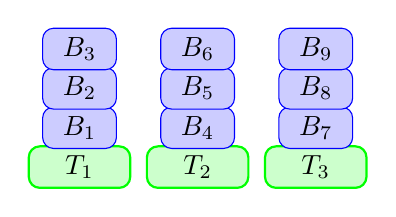
\begin{tikzpicture}[scale=0.5,auto,
block/.style ={rectangle, draw=blue, fill=blue!20,
  text width=2em, text centered, rounded corners,
  minimum height=1em
},
place/.style ={rectangle, draw=green, thick, fill=green!20,
  text width=3em, text centered, rounded corners,
  minimum height=1em
}]
\node (p1) at (0,0) [place] {$T_1$};
\node (b1) at (0,1) [block] {$B_1$};
\node (b2) at (0,2) [block] {$B_2$};
\node (b3) at (0,3) [block] {$B_3$};

\node (p2) at (3,0) [place] {$T_2$};
\node (b1) at (3,1) [block] {$B_4$};
\node (b2) at (3,2) [block] {$B_5$};
\node (b3) at (3,3) [block] {$B_6$};

\node (p2) at (6,0) [place] {$T_3$};
\node (b1) at (6,1) [block] {$B_7$};
\node (b2) at (6,2) [block] {$B_8$};
\node (b3) at (6,3) [block] {$B_9$};

\end{tikzpicture}
\caption{}\label{fig:ex6a}
\end{subfigure}%
%
\begin{subfigure}[b]{0.5\textwidth}
\centering
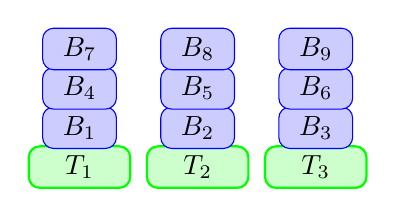
\begin{tikzpicture}[scale=0.5,auto,
block/.style ={rectangle, draw=blue, fill=blue!20,
  text width=2em, text centered, rounded corners,
  minimum height=1em
},
place/.style ={rectangle, draw=green, thick, fill=green!20,
  text width=3em, text centered, rounded corners,
  minimum height=1em
}]
\node (p1) at (0,0) [place] {$T_1$};
\node (b1) at (0,1) [block] {$B_1$};
\node (b1) at (0,2) [block] {$B_4$};
\node (b1) at (0,3) [block] {$B_7$};

\node (p2) at (3,0) [place] {$T_2$};
\node (b2) at (3,1) [block] {$B_2$};
\node (b2) at (3,2) [block] {$B_5$};
\node (b2) at (3,3) [block] {$B_8$};

\node (p2) at (6,0) [place] {$T_3$};
\node (b3) at (6,1) [block] {$B_3$};
\node (b3) at (6,2) [block] {$B_6$};
\node (b3) at (6,3) [block] {$B_9$};
\end{tikzpicture}
\caption{}\label{fig:ex6b}
\end{subfigure}%
%
\caption{Problème à 9 blocs}\label{fig:blocs_tables3}
\end{figure}

%......................................................................
  \end{exo}
  
  
%\begin{verbatim}
%;;-----------------------------------------
%;; problème #2, $FinTemps = 5, 3 blocs, 3 tables
%;;Sur(B1,T1,0) and Sur(B2,B1,0) and Sur(B3,B2,0) and Libre(B3,0) and Libre(T2,0) and Libre(T3,0)
%;;bigor $t in $Instants:
%;;  Sur(B1,T2,$t) and Sur(B2,B1,$t) and Sur(B3,B2,$t) end
%;;-----------------------------------------
%
%;;-----------------------------------------
%;; problème #3, $FinTemps = ?? au mieux, 6 blocs, 3 tables
%;; faire chercher à la main
%    Sur(B1,T1,0) and Sur(B2,T2,0) and Sur(B3,T3,0) 
%and Sur(B4,B1,0) and Sur(B5,B2,0) and Sur(B6,B3,0)
%and Sur(B7,B4,0) and Sur(B8,B5,0) and Sur(B9,B6,0)
%and Libre(B7,0) and Libre(B8,0) and Libre(B9,0)
%
%bigor $t in $Instants:
%    Sur(B1,T1,$t) and Sur(B4,T2,$t) and Sur(B7,T3,$t) 
%and Sur(B2,B1,$t) and Sur(B5,B4,$t) and Sur(B8,B7,$t)
%and Sur(B3,B2,$t) and Sur(B6,B5,$t) and Sur(B9,B8,$t)
%and Libre(B3,$t) and Libre(B6,$t) and Libre(B9,$t)
%end
%;;-----------------------------------------
%\end{verbatim}
